\documentclass{article}
\setlength{\textheight}{9.3in}
\setlength{\textwidth}{6.68in}
\setlength{\oddsidemargin}{-.20in}
\setlength{\topmargin}{-.25in}
\setlength{\headsep}{10mm}
\pagestyle{myheadings}
\usepackage{graphics}
\usepackage{epsfig}
\usepackage{multicol}
\title{\hrule \vspace{0.3cm}MLE from a Competing Risks Model of an Exponential Failure and a Lognormal Survival}
\date{10 November 2010}
\author{Nikola Chochkov, 542064 MSc Statistics HU Berlin}
\begin{document}
\maketitle
\hrule
\section{Introduction}
\indent \indent Unlike lifetime data sourced from the laboratory, lifetime data sourced from the field reflect the effects of environmental conditions and usage on a product while it is in service \cite{alam_suzuki} \cite{lawless}. Information obtained from analyzing such data thus gives manufacturers a better idea of the true reliability of their products. In this document data is considered to come from a number of items that are followed over a certain test period (eg. warranty). I assume that the data about their failure or survival, as well as the data for accumulated usage (eg. accumulated mileage for automobiles, number of hits on a computer server, number of copies for a copy-machine, etc.) has been collected for research. 
\\
\\
\indent Since the lifetime distribution of failure cases generally differs from the distribution of survivals, a two-distributional \textit{Competing risks model} is discussed here. A particular parametric form is assumed for the two lifetime distributions and an estimation approach for the parameters is suggested. Below I start with a background on the distribution selection. 
\subsection{Exponential Distribution}
\indent \indent Often failure cases of a system cannot be attributed to a defect in its design or production phase, but instead their occurrence is driven by random, unpredictable factors \cite{philips_sweeting}. They might be related to specific conditions to which the system is exposed (eg. extreme temperatures, accidents, etc). In Reliability theory failures of random type (aka abrupt failures), that occur with a constant rate over the system's lifetime, could be successfully modelled by the Exponential distribution (because of its \textit{"Memorylessness" property}). 
\\
\\
\indent Thus in this document failures are considered Exponentially distributed. In reality, of course, failures of other types need to be incorporated into the studied model as well - for example \textit{wear-out} failure types, which occur with failure rate dependent on the system's usage. A good modelling distribution for such failure modes would be for example the Weibull Distribution.  
\subsection{Lognormal Distribution}
\indent On the other hand Lognormal distribution has been shown \cite{rai_singh} to model lifetime of surviving systems. While the cited document discusses the survival of a warranty period, the distribution assumption could be used in this research without loss of generality.
\section{Competing Risks Model}
\indent \indent From now on we could without loss of generality think of automobiles as our underlying system and accumulated mileage as the collected data. More specifically we'll have the mileage at failure or mileage at survival, whichever occurs first. That's to say for each item $i$ the data we'll have will be $U_i = min(\psi_i, \eta_i)$, where $\psi$ and $\eta$ follow respectively the assumed failure and survival distributions and $\delta_i = 1$ if $i$ failed and $\delta_i = 0$ otherwise. This is known as a Competing risks model.
\\
\\
\indent The further notations and conditions of the model discussed in the document follow: 
\begin{itemize}
\item $\eta \sim Lognormal(\mu, \sigma)$ 
\item $\psi \sim Exponential(\lambda)$
\item $f_\eta(x) = \frac{1}{x \sigma \sqrt{2 \pi}} e^{-\frac{\left( \ln x - \mu \right)^2}{2\sigma^2}} = \frac{1}{x \sigma} \phi \left( \frac{\ln x - \mu}{\sigma} \right) $ is the \textit{probability densitiy function} of the Lognormal distribution, with $\phi$ being the density function of the Standard Normal Distribution
\item $\overline F_\eta(x) = 1 - \frac{1}{\sqrt{2 \pi}} e^{-\frac{\left( \ln x - \mu \right)^2}{2\sigma^2}} = \overline \Phi \left(\frac{\ln x - \mu}{\sigma}\right)$ is its \textit{survival function}, with $\overline\Phi$ being the survival function of the Standard Normal Distribution
\item $f_\psi(x) = \lambda e^{- \lambda x}$ is the \textit{pdf} of the Exponential distribution 
\item $\overline F_\psi(x) = e^{- \lambda x}$ is its \textit{survival function}
\item $n$ is the total number of units under test
\item $N_f = \{i : \delta_i = 1 \}$ (the collection of failed cases) and $n_f  = \sum_{i=1}^n \delta_i$ (i.e. $n_f = \# N_f$)
\item $N_s = \{i : \delta_i = 0 \}$ and $n_s  = n - n_f$
\item $\textbf{x}$ is the data vector and $\textbf{x} = \left[ \textbf{x}^f, \textbf{x}^s \right] = \left[ x_1^f, ... , x_{n_f}^f, x_1^s, ... , x_{n_s}^s \right] $, where:
\item $\textbf{x}^f$ is the data for failed items, $\textbf{x}^f = \left[ x_1^f, ... , x_{n_f}^f \right] $
\item $\textbf{x}^s$ is the data for survived items, $\textbf{x}^s = \left[ x_1^s, ... , x_{n_s}^s \right] $
\item $\lambda, \mu, \sigma, x > 0$
\end{itemize}
\indent We're looking for an estimation of the parameter vector ($\lambda$, $\mu$, $\sigma$)$'$ under the above model. 
\section{Maximum Likelihood Estimation }
\indent \indent We'll observe failure with probability $P(\psi < \eta) = \int_0^{\infty} f_\psi(x)\overline{F}_\eta(x) \partial x$ and we'll observe survival with probability $P(\eta < \psi) = \int_0^{\infty} f_\eta(x)\overline{F}_\psi(x) \partial x$. 
\\
\\
\indent So in our competing risks framework the density function of our variable $U$ would be $u(x) = f_\psi(x)\overline{F}_\eta(x)$ if failure and $u(x) = f_\eta(x)\overline{F}_\psi(x)$ if survival. The Likelihood function for the model could therefore be written as:
\begin{eqnarray}
L(\lambda, \mu, \sigma | \textbf{x}) &=& \prod_{i \in N_f} \left[ f_\psi \left( x_i^f \right) \overline F_\eta \left( x_i^f \right) \right]\prod_{i \in N_s} \left[ f_\eta \left( x_i^s \right) \overline F_\psi \left( x_i^s \right) \right]
\end{eqnarray}
\indent Now from the above we can derive the Log Likelihood:
\begin{eqnarray}
LogL = L^*(\lambda, \mu, \sigma | \textbf{x}) &=& \sum_{i \in N_f} \ln \left[ f_\psi(x_i^f) \right] + \sum_{i \in N_f} \ln \left[ \overline F_\eta(x_i^f) \right] + \sum_{i \in N_s} \ln \left[ f_\eta (x_i^s) \right] + \sum_{i \in N_s} \ln \left[ \overline F_\psi(x_i^s) \right]
\end{eqnarray}
\indent And if we apply the above notation and rework:
\begin{eqnarray}
L^*(\lambda, \mu, \sigma | \textbf{x}) &=& N_f \ln \lambda - \lambda \sum_{i = 1}^n x_i + \sum_{i \in N_f} \ln \overline \Phi \left( \frac{\ln x_i^f - \mu}{\sigma} \right) - \sum_{i \in N_s} \ln \sigma x_i^s + \sum_{i \in N_s} \ln \phi \left( \frac{\ln x_i^s - \mu}{\sigma} \right)
\end{eqnarray}
\indent The last equation form would be easier to work with considering the forthcoming computations involved in deriving MLEs. The estimators $\left(\hat \lambda, \hat \mu, \hat \sigma \right)'$ will namely be the values that turn $L^*$ into a maximum, so now we need to compute the \textit{Gradient} vector and \textit{Hessian} matrix in order to get them. 
\subsection{First order derivatives of $L^*$ w.r.t $\left(\lambda, \mu, \sigma \right)$}
\indent Let's denote: $z_i^{f,s} = \frac{\left(\ln x_i^{f,s} - \mu \right)}{\sigma}$. Then we derive: 
\begin{eqnarray}
\frac{\partial z}{\partial \mu} = - \frac{1}{\sigma} , \frac{\partial z} {\partial \sigma} = - \frac{1}{\sigma}z , \frac{\partial \phi}{\partial \sigma} = \frac{1}{\sigma}\phi z^2 , \frac{\partial \phi}{\partial \mu} = \frac{1}{\sigma}\phi z 
\end{eqnarray} 
\begin{eqnarray}
\frac{\partial L^*(\lambda, \mu, \sigma | \textbf{x}) }{\partial \lambda} &=& \frac{n_f}{\lambda} - \sum_{i = 1}^n x_i 
\end{eqnarray} 
\begin{eqnarray}
\frac{\partial L^*(\lambda, \mu, \sigma | \textbf{x}) }{\partial \mu} &=& \frac{1}{\sigma}\sum_{i \in N_f} \frac{\phi \left( z_i^f \right)}{\overline \Phi \left( z_i^f \right)} + \frac{1}{\sigma}\sum_{i \in N_s}z_i^s 
\end{eqnarray} 
\begin{eqnarray}
\frac{\partial L^*(\lambda, \mu, \sigma | \textbf{x}) }{\partial \sigma} &=& \frac{1}{\sigma} \sum_{i \in N_f} \frac{\phi \left( z_i^f \right) z_i^f }{\overline \Phi \left( z_i^f \right)} + \frac{1}{\sigma}\sum_{i \in N_s} (z_i^s)^2 - \frac{n_s}{\sigma} 
\end{eqnarray} 
\subsection{Second order derivatives of $L^*$ w.r.t $\left(\lambda, \mu, \sigma \right)$}\
\indent Let's denote again: $z_i^{f,s} = \frac{\left(\ln x_i^{f,s} - \mu \right)}{\sigma}$. Then we derive: 
\begin{eqnarray}
\frac{\partial^2 L^*(\lambda, \mu, \sigma | \textbf{x}) }{\partial \lambda^2} &=& - \frac{n_f}{\lambda ^ 2} 
\end{eqnarray} 
\begin{eqnarray}
\frac{\partial^2 L^*(\lambda, \mu, \sigma | \textbf{x}) }{\partial \mu^2} &=& \frac{1}{\sigma^2}\sum_{i \in N_f} \left[ \frac{\phi \left( z_i^f \right)}{\overline \Phi \left( z_i^f \right)}\left( 1 + \frac{\phi \left( z_i^f \right)}{\overline \Phi \left( z_i^f \right)} \right) z_i^f \right] - \frac{1}{\sigma^2} 
\end{eqnarray} 
\begin{eqnarray}
\frac{\partial^2 L^*(\lambda, \mu, \sigma | \textbf{x}) }{\partial \mu \partial\sigma} &=& \frac{1}{\sigma^2} \sum_{i \in N_f} \frac{\phi \left( z_i^f \right)}{\overline \Phi \left( z_i^f \right)} + \frac{1}{\sigma^2}\sum_{i \in N_f} \left[ \frac{\phi \left( z_i^f \right)}{\overline \Phi \left( z_i^f \right)}\left( 1 + \frac{\phi \left( z_i^f \right)}{\overline \Phi \left( z_i^f \right)} \right) z_i^f \right] - \frac{2}{\sigma^2}\sum_{i \in N_s} z_i^s 
\end{eqnarray} 
\begin{eqnarray}
\frac{\partial^2 L^*(\lambda, \mu, \sigma | \textbf{x}) }{\partial \sigma^2} &=& \frac{1}{\sigma^2} \sum_{i \in N_f} \left[ \frac{\phi (z_i) z_i^3}{\overline \Phi} - 2\frac{\phi(z_i)z_i}{\overline \Phi} - \frac{\phi^2(z_i) z_i^2}{\overline\Phi ^2} \right] - \frac{3}{\sigma^2}\sum_{i \in N_s} z_i^2 + \frac{n_s}{\sigma^2}
\end{eqnarray} 
\section{Simulation Studies}
\indent \indent Unfortunately the current scope of this document doesn't involve deriving the estimators in a closed form, instead I only meant to do a proof-of-concept work by means of an R simulation. However, the closed form derivation would be a certain next step for me following the good simulation results, that would help me better study the estimators properties. 
\\
\\
\indent The optimisation problem above is solved in my simulation using the R core \textit{nlminb} method, which implements Newton-Raphson numerical optimisation, for non-linear minimisation. It takes the target function, it's first derivatives vector and the hessian matrix and returns a solution vector as well as a convergency report. All simulation repetitions that I did returned positive convergence report, which is another way to verify the above computations.
\\
\\
\indent The simulation procedure itself involves the following steps.
\begin{itemize}
\item Set true parameter values for $\lambda, \mu, \sigma$. The true values are selected to make the simulation realistic. 
\item Generate two samples of size $n$ following from the Exponential and Lognormal distributions.
\item Apply the competing risks model, which would run from 1 to $n$ and on each step $i$ record the minimum from the two $i$-th realisations in the Exponential and Lognormal samples generated above. The failure or survival information is also recorded at this point.
\item Apply the calculations in section 3 and maximise the likelihood $L$ using the data from the above step. Then store the resulting estimations of the parameters.
\end{itemize}
\indent With a sample size of $n = 1000$ this procedure is performed 150 times over each of 4 different sets of true parameter values in order to obtain a histogram of the estimators' performance. Next the sample size is increased to $n = 2000$ and the simulation procedure is performed again 150 times over each of the same true parameter sets. It's expected that with the increased sample size the estimator's performance would improve.
\\
\\
\indent In the diagrams below the true values are marked with a solid blue line, whereas the mean of the estimated values is marked as a dotted red line. 
\subsection{Histograms of the estimators over 4 true parameter sets and $n$ = 1000}
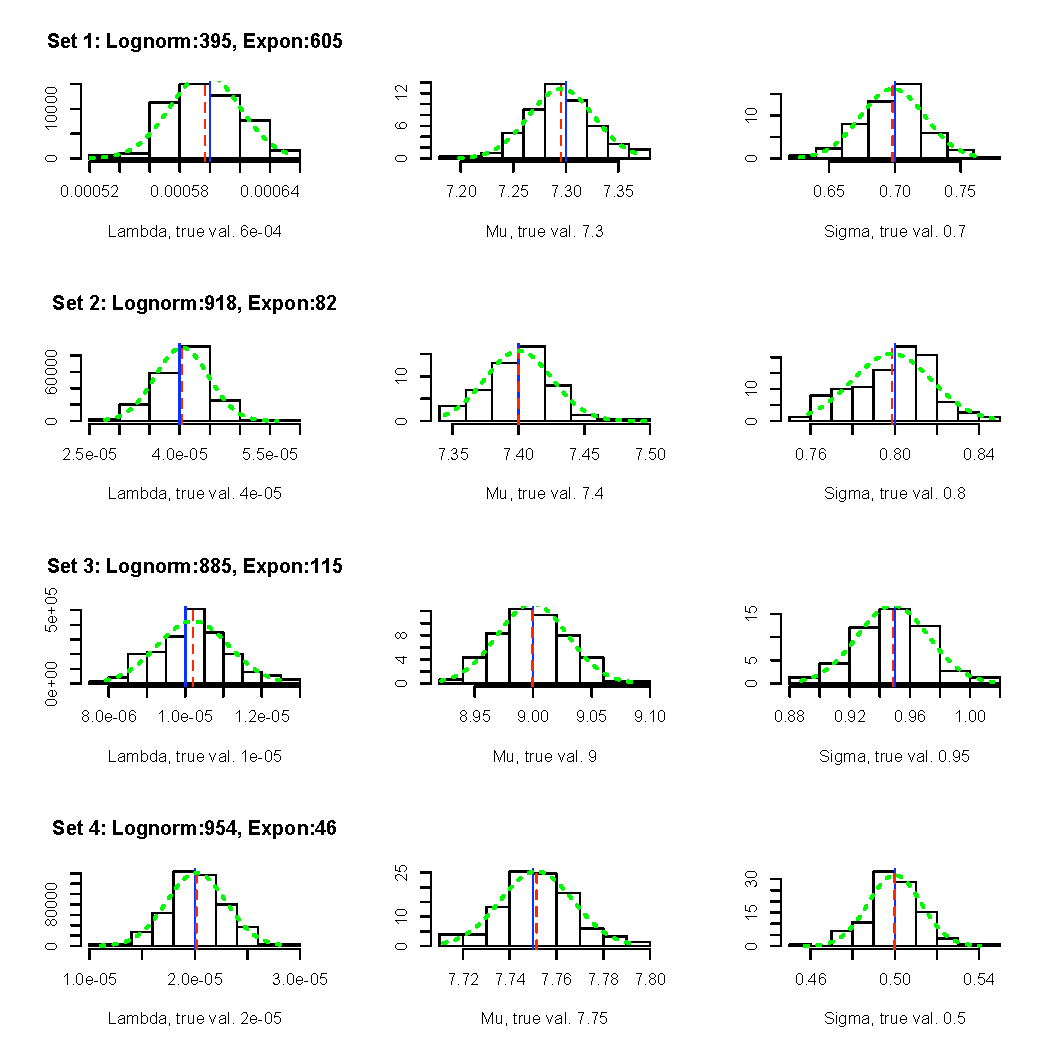
\includegraphics{Diagram1.pdf}
\subsection{Histograms at sample size $n$ = 2000}
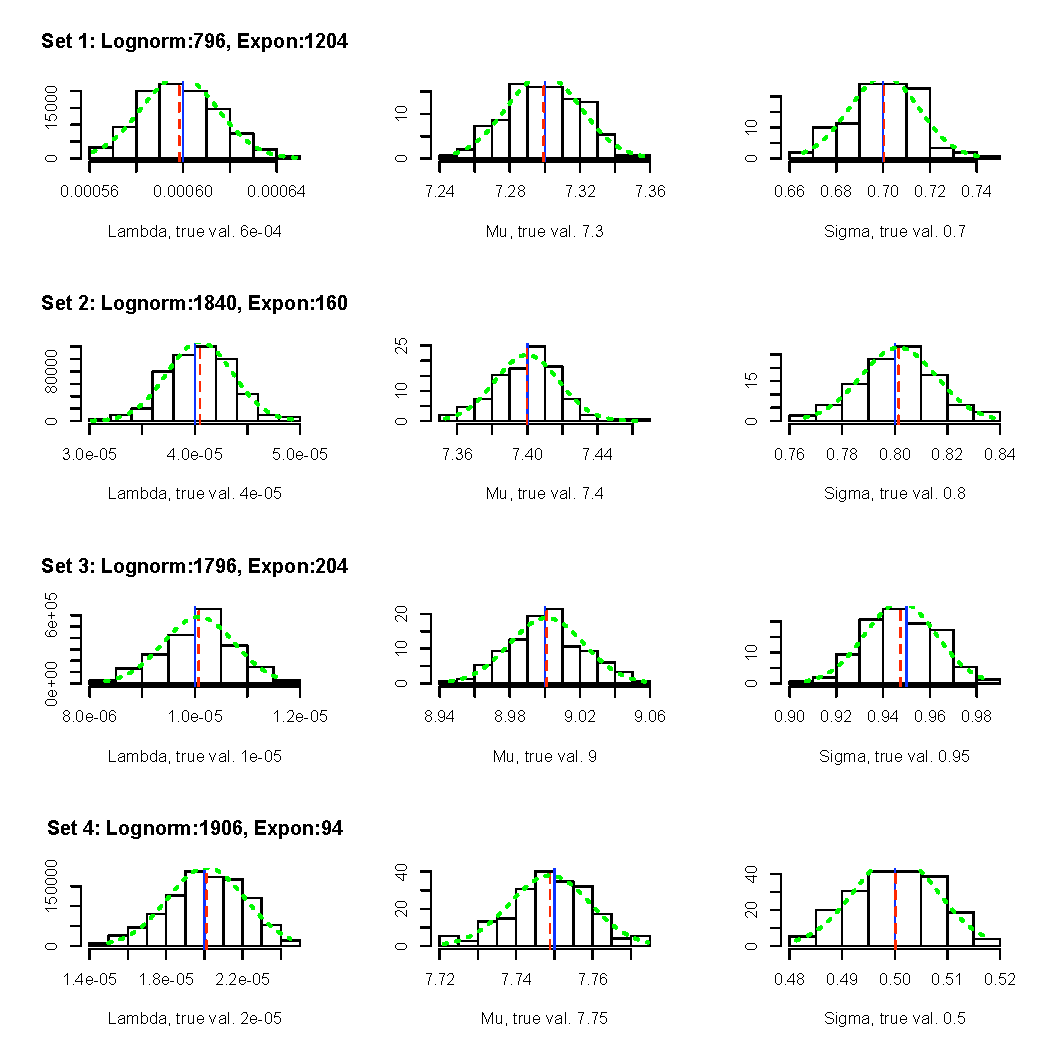
\includegraphics{Diagram2.pdf}
\section{Maximum Likelihood Estimators' properties}
This section is subject to a future progress on the matter and is for now limited to interpretation of the obtained histograms.
\subsection{Normality of the estimators.} It appears that the estimators behave normally centered around their true values. That suggests unbiasedness, which of course is to be analytically shown.  \\
\subsection{Consistency of the estimators.} Since the estimations improve over a larger sample size the consistency property is also suggested by the histograms. However this needs to be verified as well with more simulations with higher number of repetitions. As a further step I consider the derivation of the Variance-covariance matrix for the estimators vector and looking at correlation between the parameters.
\section{Next steps.}
Other than the above mentioned natural continuations of this study, I would be interested in evaluating the behaviour of the estimators on extreme cases, where for example there's just one failed item or only one survived item. The estimators' performance over very small failure or survival realisation would be very interesting because in that case there wouldn't be any other practical estimation alternative. Including a time series in the model would be another interesting extension; experimenting with different distribution assumptions, adding more failure modes to the Competing risks model, etc. etc. Finally, probably the most challenging of all would be discovering more interesting use cases fur such a model and applying it to real data.
\begin{thebibliography}{9}
\bibitem{alam_suzuki}
  Alam M.M. and Suzuki K.
  \emph{Reliability Analysis of Automobile Warranty Data Using Censoring In- formation Related to Random Failures.} 
  Proceedings of the 5th Asian Quality Congress 2007.
\bibitem{lawless}
  J. F. Lawless, X. J. Hu, and J. Cao
  \emph{Methods for the estimation of failure distributions and rates from automobile warranty data}
  Lifetime Data Analysis, vol. 1, pp. 227240, 1995. 
\bibitem{philips_sweeting}
  M. J. Philips and T. J. Sweeting
  \emph{Estimation from censored data with incomplete information}.
  Life-time Data Analysis, vol. 7, pp. 279288, 2001.
\bibitem{rai_singh}
  Rai. B. and Singh, N., 
  \emph{Customer-rush Near War- ranty Expiration Limit and Nonparametric Hazard Rate Estimation from the Known Mileage Accumu- lation Rates.}
  IEEE Transactions on Reliability, 55 (2006) 480-489.
\end{thebibliography}
\end{document}

